\documentclass{article}%
\usepackage[T1]{fontenc}%
\usepackage[utf8]{inputenc}%
\usepackage{lmodern}%
\usepackage{textcomp}%
\usepackage{lastpage}%
\usepackage{amsmath}%
\usepackage{amssymb}%
\usepackage{nccmath}%
\usepackage{hyperref}%
\usepackage{float}%
\usepackage[encoding,filenameencoding=utf8]{grffile}%
\usepackage{graphicx}%
%
\hypersetup{
    colorlinks=true,
    linkcolor=blue,
    filecolor=magenta,      
    urlcolor=cyan,
    }%
\title{Análisis de la generación de materiales no fulerenos para el mejoramiento de la eficiencia de paneles solares}%
\author{Anonymous author}%
\date{\today}%
%
\begin{document}%
\normalsize%
\maketitle%
\section{Descripción del proceso}%
\label{sec:Descripcindelproceso}%
Según lo estudiado en el artículo Design Principles and Top Non{-}Fullerene Acceptor Candidates for Organic Photovoltaics, vemos que se sigue la siguiente secuencia en la ejecución que lleva a las móleculas deseadas:%


\begin{figure}[h!]%
\centering%
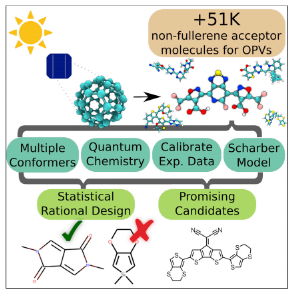
\includegraphics[width=180px]{/content/img/secuenciaArticleNo-fullerene.png}%
\caption{Secuencia del artículo}%
\end{figure}

%
Es así que a través de unas móleculas definidad con anterioridad, las cuales se encuentran en el Data S1, en el siguiente enlace https://doi.org/10.1016/j.joule.2017.10.006. Se procede a realizar con los smiles descritos en la tabla S1, una muestra de conformers, los cuales se busca su minimal local energy a través de méthodos de mecánica molecular tal como el force field, que busca la reducción de la energía total descrita en la fórmula siguiente:%
\begin{equation}
    E_{tot} = E_{str} + E_{bend} + E_{oop} + E_{tors} + E_{cross} + E_{vdw} + E_{es} 
\end{equation}%
Donde tenemos que para la stretching energy $E_{str}$ se encuentra su valor a través de la fórmula (Cabe resaltar que la siguiente fórmula no se usa en los métodos cómo MMFF94, donde se términos cuadráticos y cúbicos):%
\begin{equation}
    E_{str} = \frac{1}{2} \sum_{bonds} k_b(r-r_0)^2%
\end{equation}%
Donde:
\begin{fleqn}
\begin{equation*}
\begin{alignedat}{2}
\\ &k_b = bond-stretching \ force \ constant \\  
&r = actual\ bond\ length \\ 
&r_0 = defines\ equilibrium\ length\\
\end{alignedat}
\end{equation*}
\end{fleqn}%


\begin{figure}[H]%
\centering%
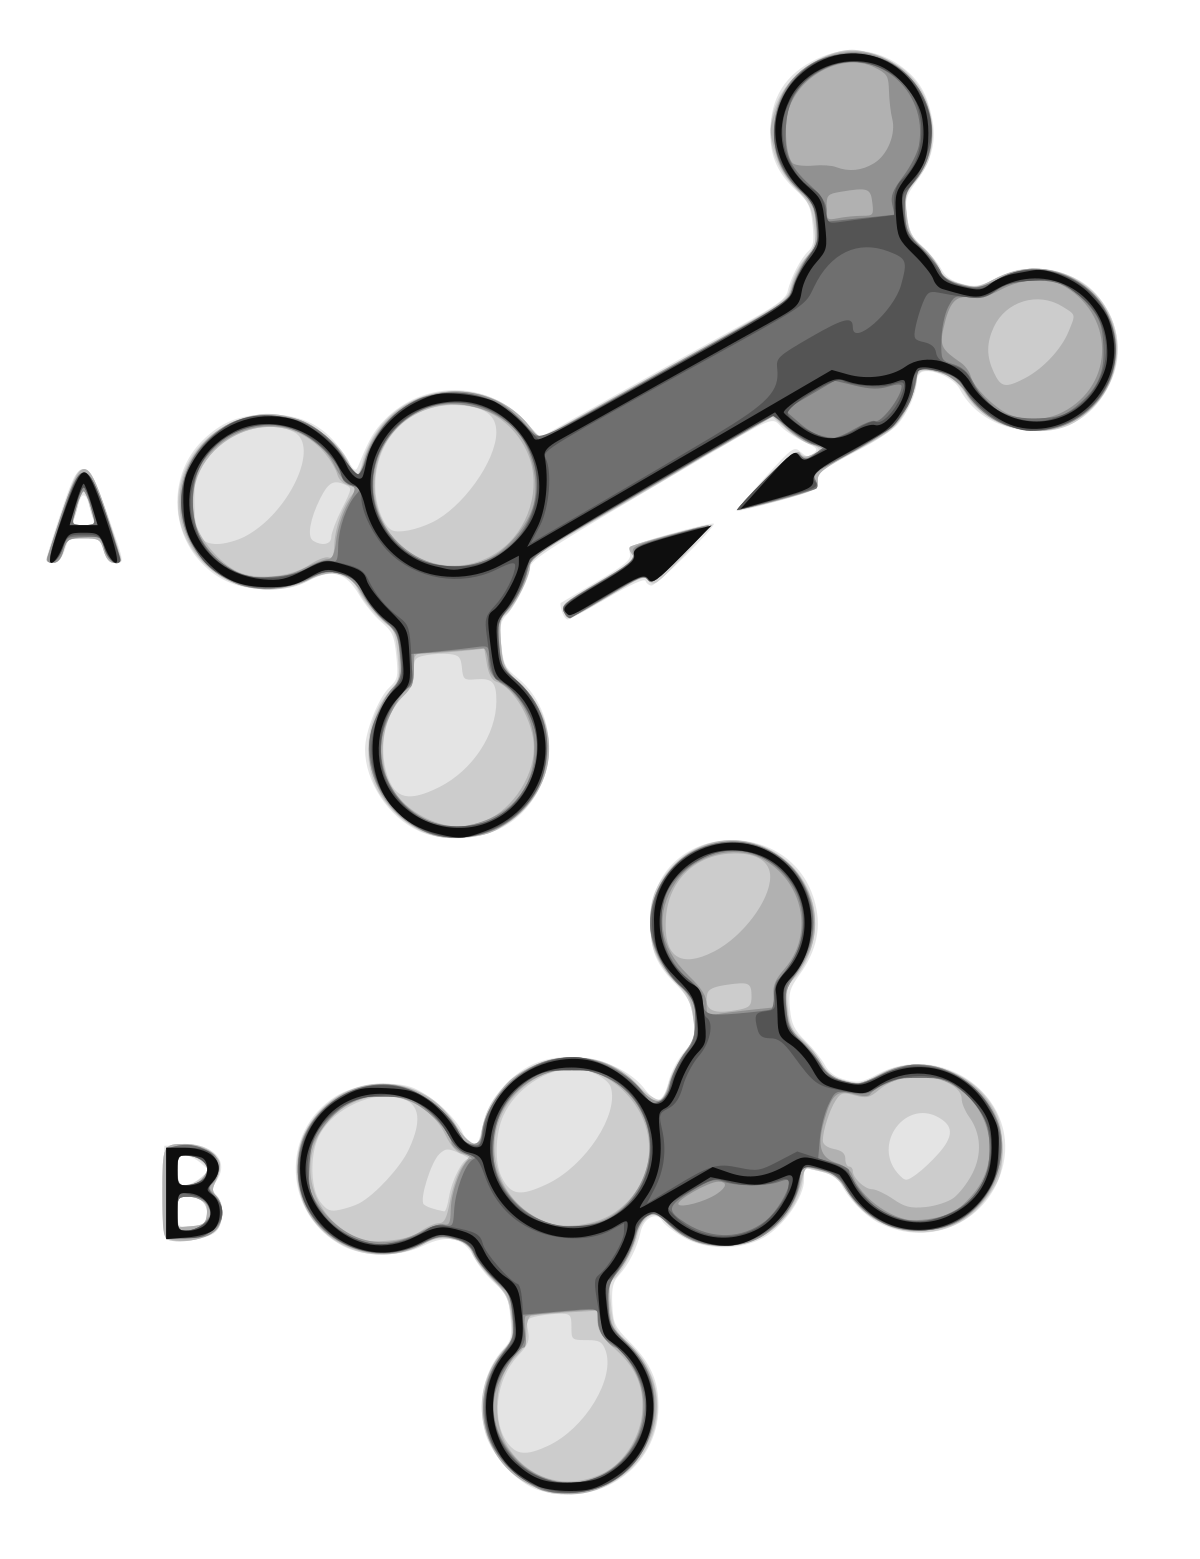
\includegraphics[width=160px]{/content/img/Bond_stretching_energy.png}%
\caption{Bond Energy}%
\end{figure}

%
Como podemos ver en la fígura 2, y por la ecuación 2, lo ideal es disminuir la longitud actual de los enlaces a la longitud de equilibrio (la biografía y método para hallarla se encuentra en el siguiente \href{https://chem.libretexts.org/Bookshelves/Physical_and_Theoretical_Chemistry_Textbook_Maps/Supplemental_Modules_(Physical_and_Theoretical_Chemistry)/Chemical_Bonding/Fundamentals_of_Chemical_Bonding/Bond_Order_and_Lengths}{enlace}. Ahora para la Angle Bending Energy, $E_{bend}$ se encuentra su valor a través de la fórmula:%
\begin{equation}
    E_{bend} = \frac{1}{2} \sum_{angles} k_\theta (\theta - \theta_0)^2
\end{equation}%


\begin{figure}[H]%
\centering%
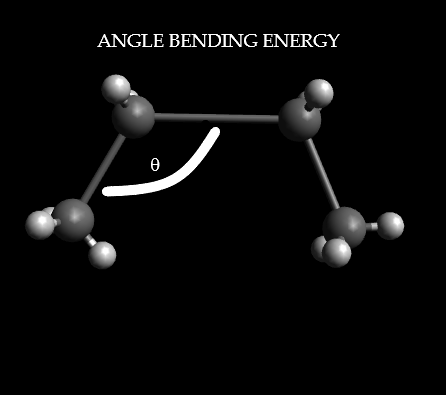
\includegraphics[width=180px]{/content/img/angleBending.png}%
\caption{Bond Energy}%
\end{figure}

%
\section{Preguntas}%
\label{sec:Preguntas}%
¿La razón por la cual se crean conformers en un inicio, es para dar diferentes configuraciones desde las cuales al aplicar el MMFF se logre una mayor probabilidad de encontrar el mínimo global de la energía?

%
\end{document}